% Options for packages loaded elsewhere
\PassOptionsToPackage{unicode}{hyperref}
\PassOptionsToPackage{hyphens}{url}
\PassOptionsToPackage{dvipsnames,svgnames,x11names}{xcolor}
%
\documentclass[
  number]{elsarticle}

\usepackage{amsmath,amssymb}
\usepackage{iftex}
\ifPDFTeX
  \usepackage[T1]{fontenc}
  \usepackage[utf8]{inputenc}
  \usepackage{textcomp} % provide euro and other symbols
\else % if luatex or xetex
  \usepackage{unicode-math}
  \defaultfontfeatures{Scale=MatchLowercase}
  \defaultfontfeatures[\rmfamily]{Ligatures=TeX,Scale=1}
\fi
\usepackage{lmodern}
\ifPDFTeX\else  
    % xetex/luatex font selection
\fi
% Use upquote if available, for straight quotes in verbatim environments
\IfFileExists{upquote.sty}{\usepackage{upquote}}{}
\IfFileExists{microtype.sty}{% use microtype if available
  \usepackage[]{microtype}
  \UseMicrotypeSet[protrusion]{basicmath} % disable protrusion for tt fonts
}{}
\makeatletter
\@ifundefined{KOMAClassName}{% if non-KOMA class
  \IfFileExists{parskip.sty}{%
    \usepackage{parskip}
  }{% else
    \setlength{\parindent}{0pt}
    \setlength{\parskip}{6pt plus 2pt minus 1pt}}
}{% if KOMA class
  \KOMAoptions{parskip=half}}
\makeatother
\usepackage{xcolor}
\setlength{\emergencystretch}{3em} % prevent overfull lines
\setcounter{secnumdepth}{5}
% Make \paragraph and \subparagraph free-standing
\ifx\paragraph\undefined\else
  \let\oldparagraph\paragraph
  \renewcommand{\paragraph}[1]{\oldparagraph{#1}\mbox{}}
\fi
\ifx\subparagraph\undefined\else
  \let\oldsubparagraph\subparagraph
  \renewcommand{\subparagraph}[1]{\oldsubparagraph{#1}\mbox{}}
\fi


\providecommand{\tightlist}{%
  \setlength{\itemsep}{0pt}\setlength{\parskip}{0pt}}\usepackage{longtable,booktabs,array}
\usepackage{calc} % for calculating minipage widths
% Correct order of tables after \paragraph or \subparagraph
\usepackage{etoolbox}
\makeatletter
\patchcmd\longtable{\par}{\if@noskipsec\mbox{}\fi\par}{}{}
\makeatother
% Allow footnotes in longtable head/foot
\IfFileExists{footnotehyper.sty}{\usepackage{footnotehyper}}{\usepackage{footnote}}
\makesavenoteenv{longtable}
\usepackage{graphicx}
\makeatletter
\def\maxwidth{\ifdim\Gin@nat@width>\linewidth\linewidth\else\Gin@nat@width\fi}
\def\maxheight{\ifdim\Gin@nat@height>\textheight\textheight\else\Gin@nat@height\fi}
\makeatother
% Scale images if necessary, so that they will not overflow the page
% margins by default, and it is still possible to overwrite the defaults
% using explicit options in \includegraphics[width, height, ...]{}
\setkeys{Gin}{width=\maxwidth,height=\maxheight,keepaspectratio}
% Set default figure placement to htbp
\makeatletter
\def\fps@figure{htbp}
\makeatother

\makeatletter
\makeatother
\makeatletter
\makeatother
\makeatletter
\@ifpackageloaded{caption}{}{\usepackage{caption}}
\AtBeginDocument{%
\ifdefined\contentsname
  \renewcommand*\contentsname{Table of contents}
\else
  \newcommand\contentsname{Table of contents}
\fi
\ifdefined\listfigurename
  \renewcommand*\listfigurename{List of Figures}
\else
  \newcommand\listfigurename{List of Figures}
\fi
\ifdefined\listtablename
  \renewcommand*\listtablename{List of Tables}
\else
  \newcommand\listtablename{List of Tables}
\fi
\ifdefined\figurename
  \renewcommand*\figurename{Figure}
\else
  \newcommand\figurename{Figure}
\fi
\ifdefined\tablename
  \renewcommand*\tablename{Table}
\else
  \newcommand\tablename{Table}
\fi
}
\@ifpackageloaded{float}{}{\usepackage{float}}
\floatstyle{ruled}
\@ifundefined{c@chapter}{\newfloat{codelisting}{h}{lop}}{\newfloat{codelisting}{h}{lop}[chapter]}
\floatname{codelisting}{Listing}
\newcommand*\listoflistings{\listof{codelisting}{List of Listings}}
\makeatother
\makeatletter
\@ifpackageloaded{caption}{}{\usepackage{caption}}
\@ifpackageloaded{subcaption}{}{\usepackage{subcaption}}
\makeatother
\makeatletter
\@ifpackageloaded{tcolorbox}{}{\usepackage[skins,breakable]{tcolorbox}}
\makeatother
\makeatletter
\@ifundefined{shadecolor}{\definecolor{shadecolor}{rgb}{.97, .97, .97}}
\makeatother
\makeatletter
\makeatother
\makeatletter
\makeatother
\ifLuaTeX
  \usepackage{selnolig}  % disable illegal ligatures
\fi
\usepackage[]{natbib}
\bibliographystyle{elsarticle-num}
\IfFileExists{bookmark.sty}{\usepackage{bookmark}}{\usepackage{hyperref}}
\IfFileExists{xurl.sty}{\usepackage{xurl}}{} % add URL line breaks if available
\urlstyle{same} % disable monospaced font for URLs
\hypersetup{
  pdftitle={Interactive Visualization Framework for Forensic Bullet Comparisons},
  pdfauthor={Nathan Rethwisch; Heike Hofmann},
  pdfkeywords={Land engraved area, Forensic Pattern
Analysis, Topographic Microscopy, 3d Imaging, Statistics, Machine
learning, Interactive Forensic Modeling},
  colorlinks=true,
  linkcolor={blue},
  filecolor={Maroon},
  citecolor={Blue},
  urlcolor={Blue},
  pdfcreator={LaTeX via pandoc}}

\setlength{\parindent}{6pt}
\begin{document}

\begin{frontmatter}
\title{Interactive Visualization Framework for Forensic Bullet
Comparisons}
\author[1]{Nathan Rethwisch%
%
}
 \ead{nreth@iastate.edu} 
\author[1]{Heike Hofmann%
%
}
 \ead{hofmann@iastate.edu} 

\affiliation[1]{organization={Center for Statistics and Applications in
Forensic Evidence (CSAFE), Iowa State
University},city={Ames},country={United
States},countrysep={,},postcode={50011},postcodesep={}}

\cortext[cor1]{Corresponding author}


        





\begin{keyword}
    Land engraved area \sep Forensic Pattern Analysis \sep Topographic
Microscopy \sep 3d Imaging \sep Statistics \sep Machine learning \sep 
    Interactive Forensic Modeling
\end{keyword}
\end{frontmatter}
    \ifdefined\Shaded\renewenvironment{Shaded}{\begin{tcolorbox}[borderline west={3pt}{0pt}{shadecolor}, boxrule=0pt, sharp corners, breakable, interior hidden, enhanced, frame hidden]}{\end{tcolorbox}}\fi

\makeatletter
\def\ps@pprintTitle{%
  \let\@oddhead\@empty
  \let\@evenhead\@empty
  \def\@oddfoot{\reset@font\hfil\thepage\hfil}
  \let\@evenfoot\@oddfoot
}
\makeatother

\hypertarget{introduction}{%
\section{Introduction}\label{introduction}}

Impressions left on fired bullets, known as Land Engraved Areas (LEAs),
are crucial in forensic analyses to establish whether two discharged
bullets originated from the same firearm barrel. Current practices rely
on forensic examiners to manually assess similarity based on visual
comparisons. This analysis can be aided through algorithmic comparisons,
which rely on 3D topographic imaging to evaluate matching bullets. This
presented work adds to that algorithmic framework by creating a
visualization diagnostic tool to assess how accurate the predictions
are. The framework is used to analyze a real-world case of mislabeled
bullet scans.

\hypertarget{houston-persistence-data}{%
\subsection{Houston Persistence Data}\label{houston-persistence-data}}

The data used for this study comes from a set of 40 fired bullets in a
Houston lab. 13 different firearms were used for the study, each being
the same make and model. The first ten (firearms A-J) were produced
consecutively, while the other three (firearms 1-3) were selectived
randomly. For each firearm, 40 bullets were fired and collected. For
each of the 40 bullets, there were six LEAs captured via topographic
imaging. These LEAs are what are used for the analysis.

Therefore, the structure of the data is as follows:

\begin{itemize}
\tightlist
\item
  13 firearms

  \begin{itemize}
  \tightlist
  \item
    For each firearm, 40 bullets

    \begin{itemize}
    \tightlist
    \item
      For each bullet, 6 images of Land Engraved Areas
    \end{itemize}
  \end{itemize}
\end{itemize}

\hypertarget{algorithmic-comparisons}{%
\section{Algorithmic Comparisons}\label{algorithmic-comparisons}}

The basis for algorithmic comparison is comparing two of these LEA
images, shown in figure 1.The base of the bullet is seen at the bottom
of the image, with the bullet curving from left to right.

\begin{figure}[H]

{\centering \includegraphics{../figure/unnamed-chunk-4-1.png}

}

\caption{Two Land Engraved Images Side-by-Size}

\end{figure}

The steps to comparing these two images are as follows for all
non-damaged scans:

\begin{enumerate}
\def\labelenumi{\arabic{enumi}.}
\tightlist
\item
  A cross-section is identified on the bullet. This cross-section is the
  lowest possible horizontal line that does not pass through any
  breakoff in the bullet.
\item
  Topographical measurement from this crosscut are used to create a
  signature. The ends of the signature are removed to account for the
  curve of the bullet. This is shown in figure 2.
\end{enumerate}

\begin{figure}[H]

{\centering 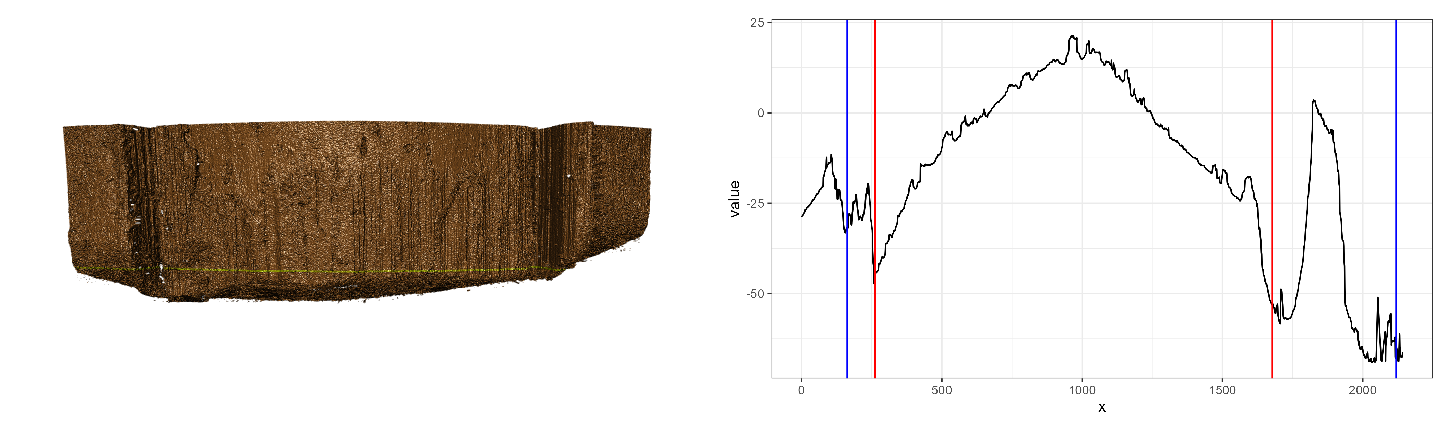
\includegraphics{../figure/unnamed-chunk-3-1.png}

}

\caption{Crosscut Signature Derived From LEA}

\end{figure}

\begin{enumerate}
\def\labelenumi{\arabic{enumi}.}
\setcounter{enumi}{2}
\tightlist
\item
  After generating signatures for multiple lands engraved areas, the two
  signatures are aligned with each other. This is shown in figure 3.
\end{enumerate}

\begin{figure}[H]

{\centering 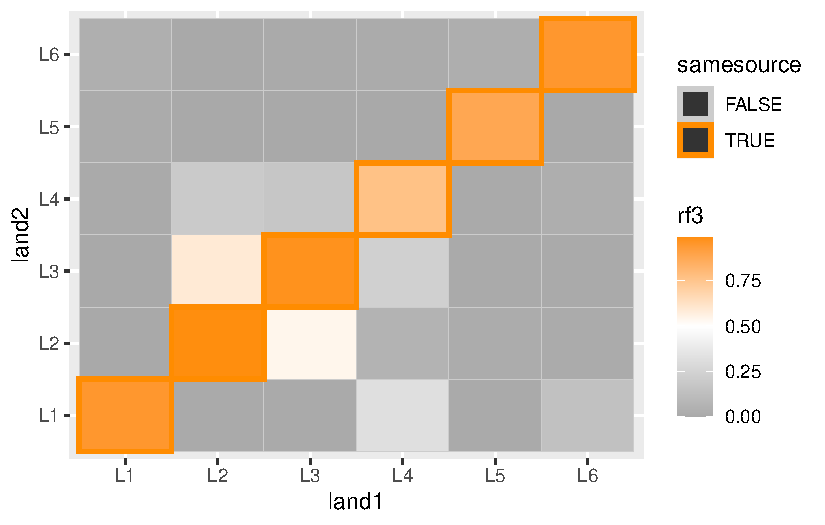
\includegraphics{"../figure/unnamed-chunk-6-1.png"}

}

\caption{Aligned Signatures of Two Bullets}

\end{figure}

\begin{enumerate}
\def\labelenumi{\arabic{enumi}.}
\setcounter{enumi}{3}
\tightlist
\item
  Aligned signatures are compared using a cross-correlation function.
  This gives a number that can be used to assess how similar the lands
  are.
\item
  Because there are six lands per bullet, to compare two bullets to each
  other, all six lands from one bullet are compared to all six from
  another bullet. This creates for 36 total comparisons. Figure 4 shows
  these comparisons, with orange indicating a higher correlation and
  grey indicating low correlation. Bullets that match, such as this one,
  are expected to have six areas of high correlation for the six matches
  and 30 areas of low correlation for the 30 non-matches.
\end{enumerate}

\begin{figure}[H]

{\centering \includegraphics[width=\textwidth,height=0.4\textheight]{../docs/Land-to-Land Grids/Barrel A/BA-B32-B32.png}

}

\caption{Comparing Correlation Scores Across Two Bullets}

\end{figure}

Further information about this process is explained in \emph{citation}

\hypertarget{interactive-html-visualization-tool}{%
\section{Interactive HTML Visualization
Tool}\label{interactive-html-visualization-tool}}

\hypertarget{intrafirearm-comparisons}{%
\subsection{Intrafirearm Comparisons}\label{intrafirearm-comparisons}}

With a use case with multiple bullets, such as in the Houston
Persistence data, it is beneficial to visualize the comparisons across
all bullet-to-bullet comparisons for a firearm. This allows users to
assess model accuracy, analyze why certain bullets may not be performing
well, and look for areas of poor performance. To achieve this, we
calculated a phase score for each bullet-to-bullet comparison. For each
bullet-to-bullet comparison, the phase score is the mean cross
correlation score of the six lands that match between the two bullets
minus the mean score of the thirty non-matches. \[ 
  phase\_ccf\_score = \frac{mean(ccf\_matches)}{mean(ccf\_non\_matches)}
\] *Note: In this case, ccf = cross-correlation function.

This phase ccf score was calculated across all \[40 * 40 = 1600\]
bullet-to-bullet comparisons, and then plotted in figure 5.

\begin{figure}[H]

{\centering 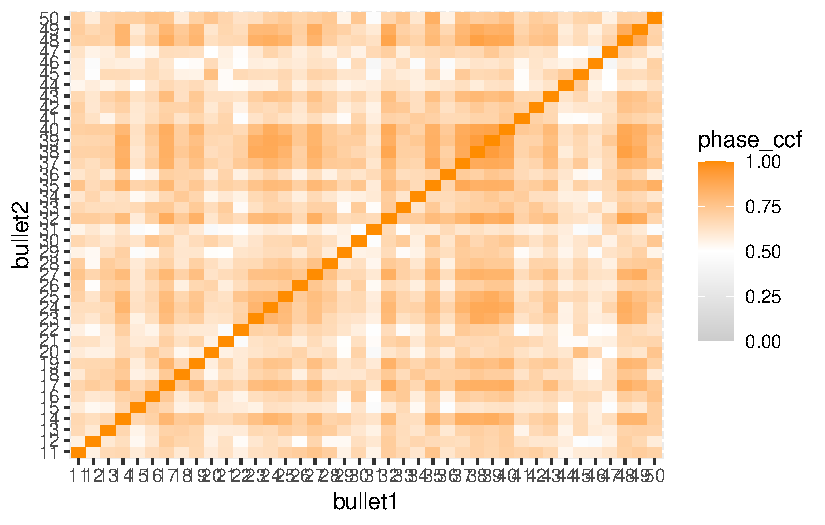
\includegraphics{Interactive-Visualization-Framework_files/figure-pdf/unnamed-chunk-2-1.pdf}

}

\caption{Intrabarrel Comparisons between phase\_ccf scores}

\end{figure}

We took this a step further by creating an interactive framework to
analyze the entire steps of the process - from image creation to the
barrel-to-barrel grid. This file starts with the barrel-to-barrel grid,
as shown in figure 5. When the user clicks on a particular square in the
grid, it directs to the appropriate comparison grid between the two
barrels, as shown in figure 4. Then, the user can click on a particular
square within that grid to query information on the lands used in the
land-to-land comparison, including the images, selected crosscut, and
aligned signatures. This framework is shown in figure 6.

\begin{figure}[H]

{\centering 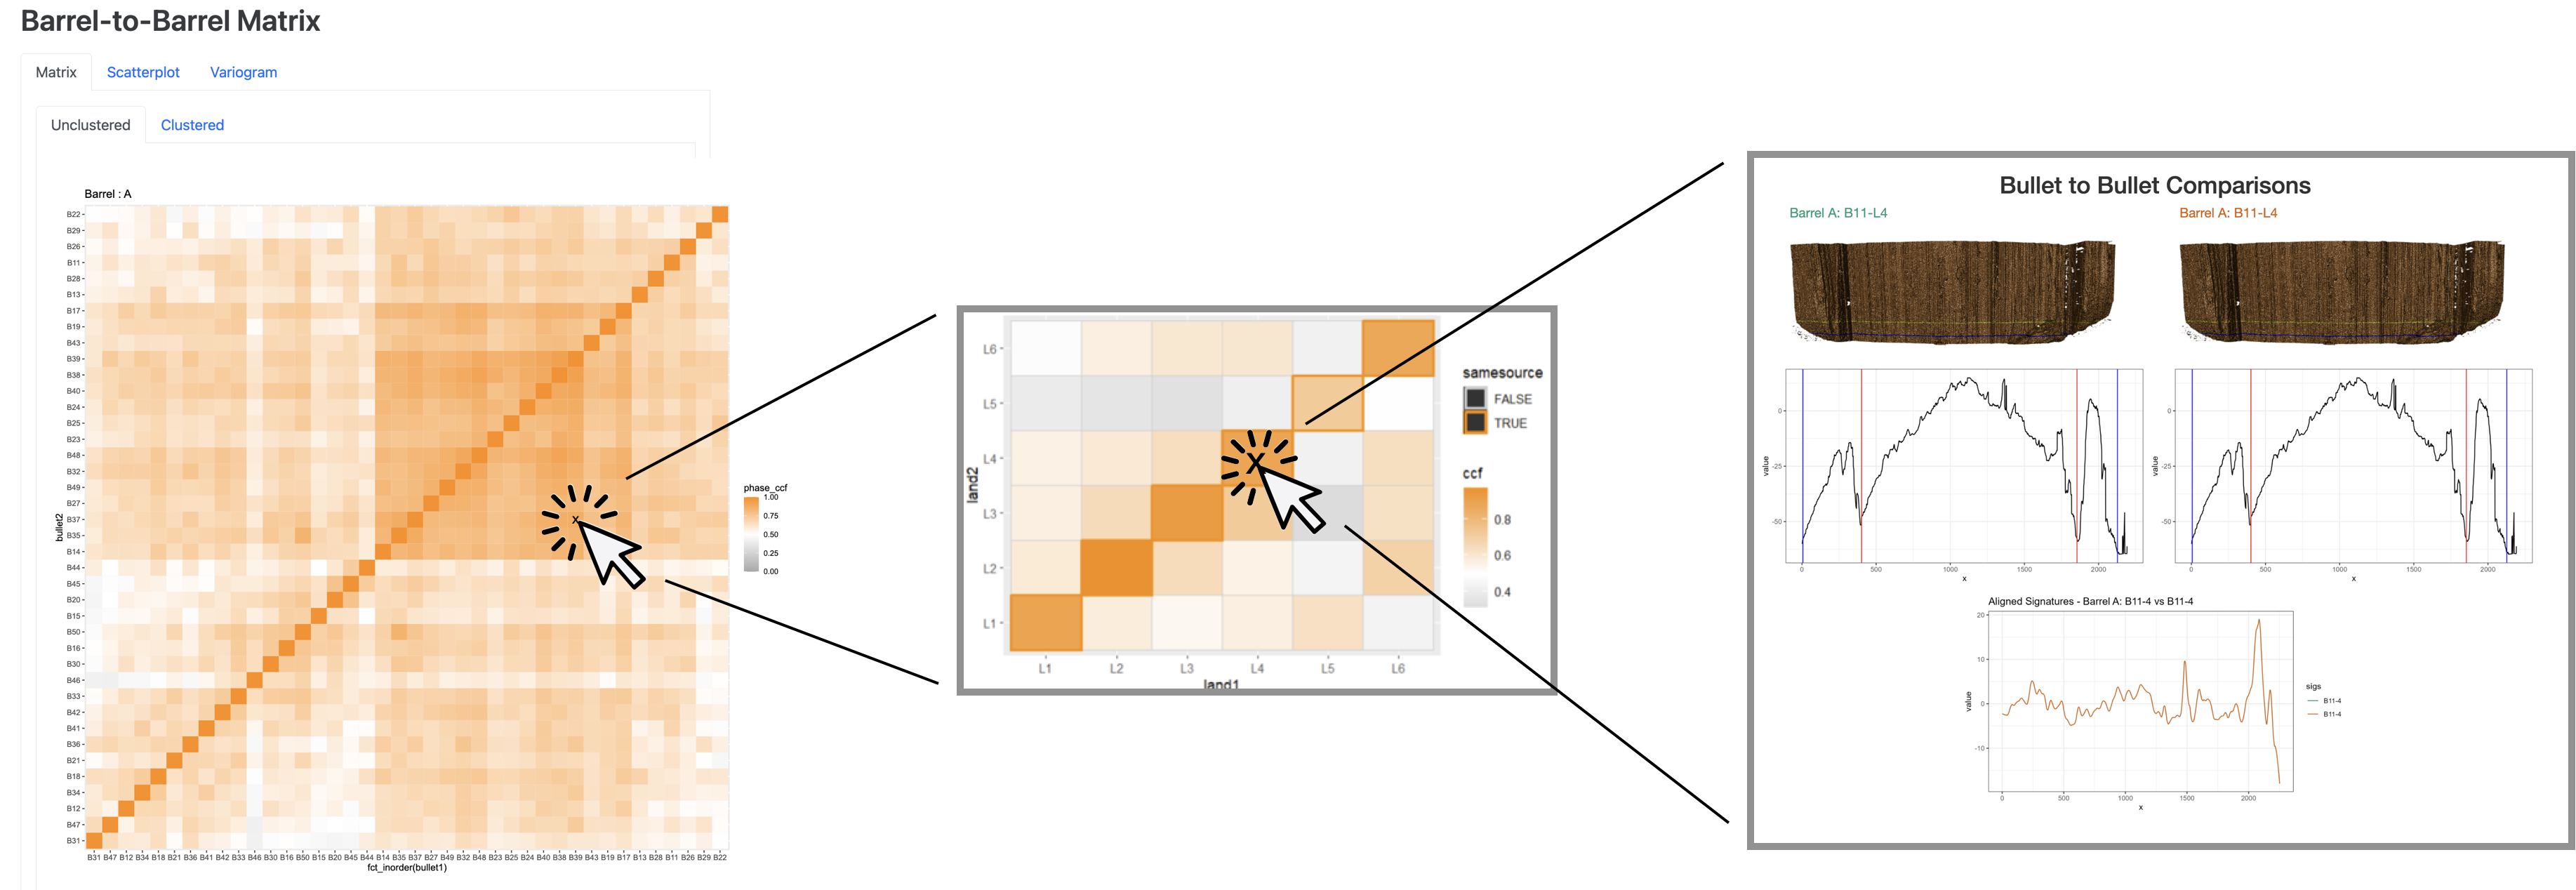
\includegraphics{../figure/overview.png}

}

\caption{Interactive Framework Covering Bullet Comparison Algorithm}

\end{figure}

This framework allows the user to quickly identify problematic areas
that may cause prediction performance to suffer. By showing all steps of
the algorithm, not only can users that a problem has occurred, but it
allows them to pinpoint that specific problem to a particular step in
the algorithmic process.

\hypertarget{a-real-use-case---incorrectly-labelled-scans}{%
\section{A Real Use Case - Incorrectly Labelled
Scans}\label{a-real-use-case---incorrectly-labelled-scans}}

A real world use-case of this framework comes from the
Houston-Persistence dataset. After rending the bullet-to-bullet
comparisons for firearm D, it became immediately apparent that there was
an error in the analysis for bullets 35-40. These bullets performed well
with each other, but did not score highly in comparison to the other
bullets shot from this firearm, as shown in figure 7.

\begin{figure}[H]

{\centering 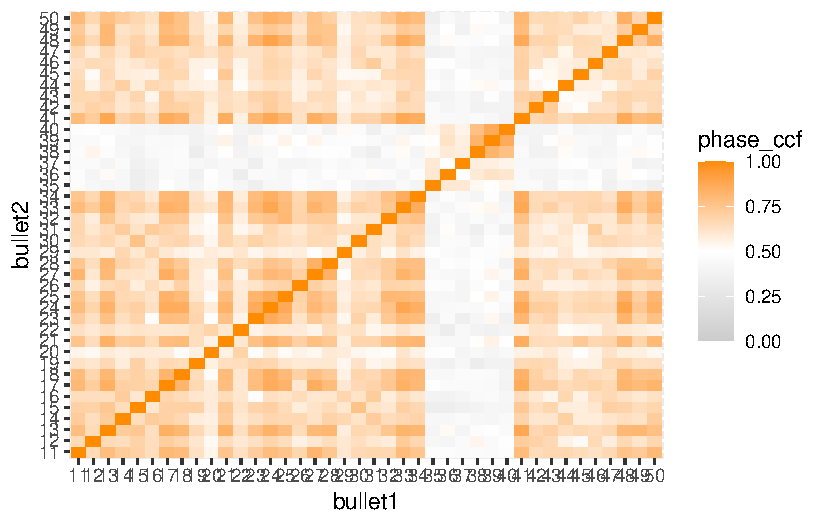
\includegraphics{Interactive-Visualization-Framework_files/figure-pdf/unnamed-chunk-3-1.pdf}

}

\caption{Bullet-to-Bullet Comparisons - Firearm D}

\end{figure}

\hypertarget{rescans}{%
\subsection{Rescans}\label{rescans}}

The first course of action was to redo the 3D topographical imaging
performed on the bullets in question. To have a baseline, bullets 33-36
were rescanned. Bullets 33 and 34 represent scans that were already
producing expected results, while bullet 35 and 36 represent two bullets
that are performing poorly.

\hypertarget{grooves}{%
\subsubsection{Grooves}\label{grooves}}

One reason why the bullets may be performing poorly is due to the
groove-engraved areas being scanned in instead of the land-engraved
areas. When firearms are produced, a metal rod is used to clean the
inside of the produced barrel. This rod smooths rougher areas in the
barrel and often creates less evident topographical differences. The
problem with using grooves for analysis is that they do not differ
between barrels - the pattern is unique to the rod used and thus cannot
link a bullet to a specific firearm. When analyzing the images of the
grooves manually, it quickly became apparent that this was not the cause
of the problem. The left figure below shows the original scan from
Bullet 35, while the right figure shows a rescanned groove for that same
data. Visually, the rescanned groove has much less topographical
protrusions in comparison to the original image.

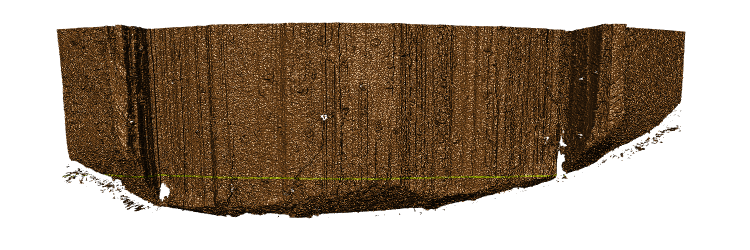
\includegraphics[width=0.49\textwidth,height=\textheight]{../images/Barrel D/HFSCP-BD-B35-L2.png}
\includegraphics[width=0.49\textwidth,height=\textheight]{../images/HFSCP-BD2-B33-G2.png}

When replacing bullets 33-36 in the original data with the rescanned
grooves, this visual comparison is enforced with the phase\_ccf data.
Figure 8 shows the intrafirearm matrix when replacing bullets 33-36.

\begin{figure}[H]

{\centering \includegraphics{Interactive-Visualization-Framework_files/figure-pdf/unnamed-chunk-4-1.pdf}

}

\caption{Intrafirearm Matrix With Rescanned Grooves}

\end{figure}

Not only are bullets 35 and 36 performing worse than before, the scores
on bullet 33 and 34, the bullets who originally had good performance,
has declined significantly. Thus, we can conclude that the innacuracy of
the original data is not because groove areas were used instead of
lands.

\hypertarget{lands}{%
\subsubsection{Lands}\label{lands}}

Next, we compared the rescanned lands to the original scans. While it
was hard to draw similarities between the visual images, they were not
as drastically different as when comparing to the grooves in the
previous step. However, when we replaced bullets 33-36 with the rescans,
as show in Figure 9, the performance of the affected bullets was on par
with the rest of the bullets shot by firearm D.

\begin{figure}[H]

{\centering 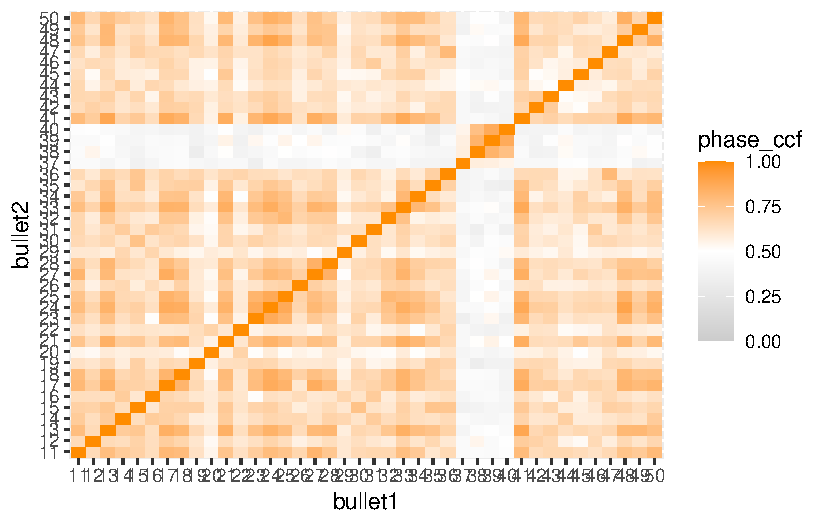
\includegraphics{Interactive-Visualization-Framework_files/figure-pdf/unnamed-chunk-5-1.pdf}

}

\caption{Rescans of Lands Replacing Bullets 33-36 of Barrel D}

\end{figure}

Therefore, we can conclude that the rescans are accurate to the true
lands from barrel D. This means that the cause of the original
inaccuracy is not attributed to the model, but instead is likely cause
by mislabelling or inadeuqate scnas.

\hypertarget{comparing-other-bullets}{%
\subsection{Comparing Other Bullets}\label{comparing-other-bullets}}

The next step was to see if the scans came from another firearm in the
dataset and were simply mislabelled. We selected one bullet from each
firearm that performed exceptionally when compared to the other bullets
from that same firearm (12 bullets in total). Those bullets were then
compared to both each other and bullet 39 from firearm. D, one of the
poor performing bullets when compared to other in that firearm.

We found that in 11 of the 12 bullets, they performed poor when compared
to the bullet from firearm D. The exception to this rule was the bullet
selected from firearm C. When comparing that bullet to bullet 39 of
barrel D, the algorithm showed that the two bullets were likely fired
from the same firearm, as shown in Figure 10.

\begin{figure}[H]

{\centering 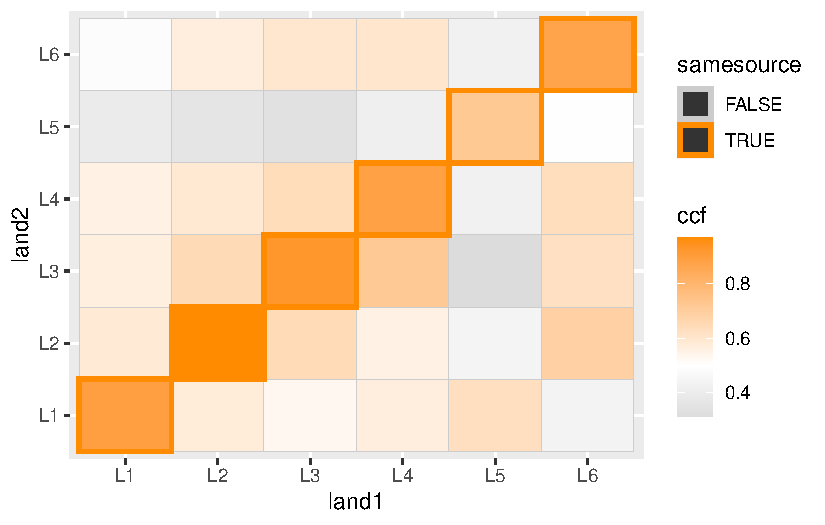
\includegraphics{Interactive-Visualization-Framework_files/figure-pdf/unnamed-chunk-7-1.pdf}

}

\caption{Comparison of Bullet From Firearm C and Bullet 39 of Firearm D}

\end{figure}

It is also important to note that the selected bullets did not perform
well when compared with each other (i.e.~- the bullet from Firearm A did
not match the bullet from Firearm B). This means that the similarity
between the bullet from Firearm C and the poor-performing bullet from
firearm D cannot be attributed to well-performing bullets being accurate
with other firearms. Thus, we have strong evidence that the bullets were
mislabeled and poor-performing bullets actually belong to barrel C.
Replace the comparisons in barrel C with barrels 35-40 that were
originally labelled barrel D is shown in Figure 11:

\begin{figure}[H]

{\centering 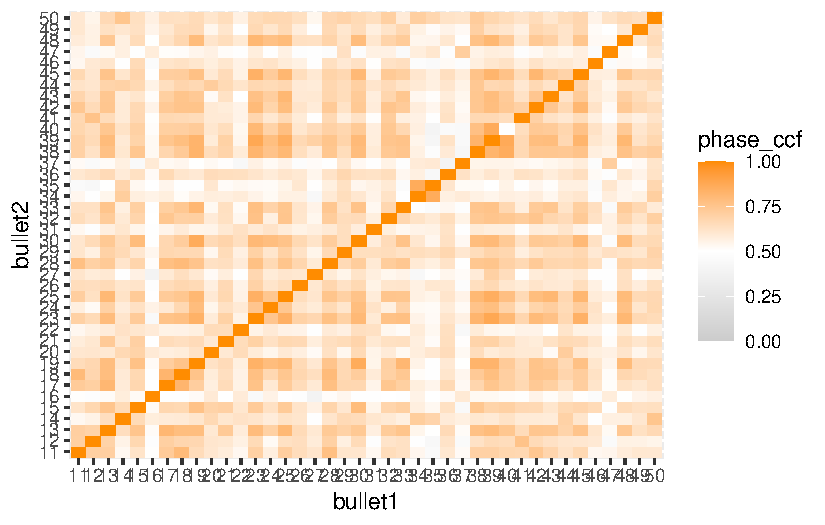
\includegraphics{Interactive-Visualization-Framework_files/figure-pdf/unnamed-chunk-8-1.pdf}

}

\caption{Replacing Barrel C Scans with Poor Performing Scans Labelled
Barrel D}

\end{figure}

Although it looks like maybe there is a dip in performance, it is
important to note that we are not replacing bullets 34-37, where the
model seems to have a somewhat weaker performance. Instead, we are
replacing bullets 35-40, which have little effect on overall model
performance. This point is emphasized when compared to the original
bullet-to-bullet matrix for firearm C, as shown in figure 12.

\begin{figure}[H]

{\centering 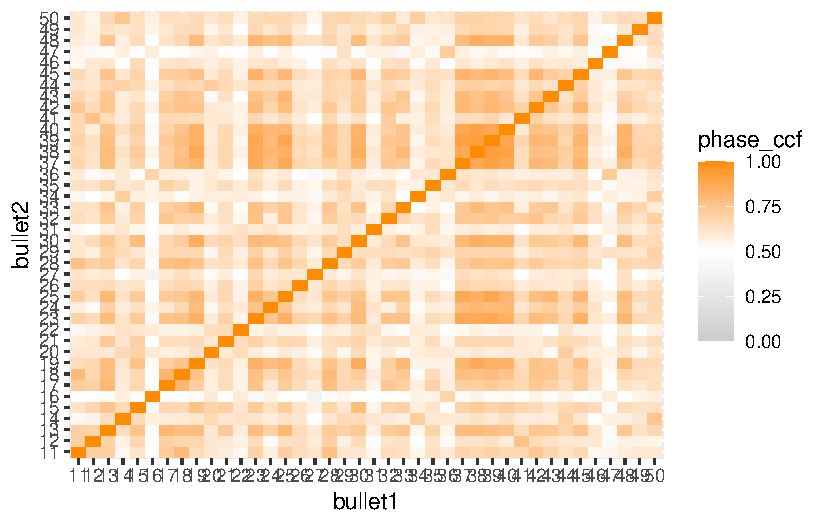
\includegraphics{Interactive-Visualization-Framework_files/figure-pdf/unnamed-chunk-9-1.pdf}

}

\caption{Bullet-to-bullet matrix for firearm C}

\end{figure}

There is somewhat of a difference in bullet 37, but overall these scans
perform very well when compared to other bullets shot by firearm C.
Thus, we can conclude that bullets 35-40 were mislabelled and were shot
by firearm C, not D.

\hypertarget{comparison-to-old-scans}{%
\subsection{Comparison to Old Scans}\label{comparison-to-old-scans}}

To further support this claim, we decided to compare the old scans to
the new rescans for barrel D. If our theory is true, bullets 33 and 34
should match because the come from the same source. However, bullets 35
and 36 should not match because the old scans come from firearm C and
the newscans come from firearm D. Figure 13 shows this comparison.

\begin{figure}[H]

{\centering 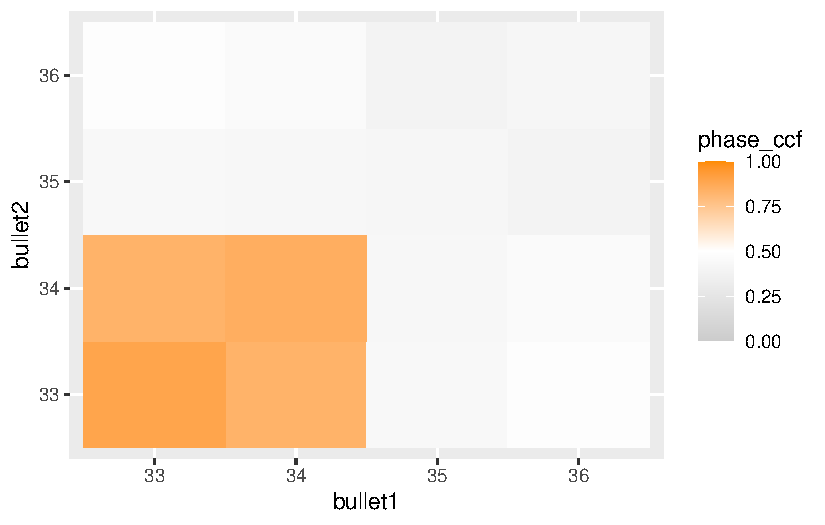
\includegraphics[width=0.5\textwidth,height=0.5\textheight]{Interactive-Visualization-Framework_files/figure-pdf/unnamed-chunk-10-1.pdf}

}

\caption{Replacing Barrel C Scans with Poor Performing Scans Labelled
Barrel D}

\end{figure}

We see the expected outcome. Therefore, we are confident that these
scans do not come from the same source, and can be attributed to
mislabelling.

\hypertarget{conclusion}{%
\section{Conclusion}\label{conclusion}}

This paper presented an interactive framework for analyzing algorithmic
comparisons of whether two bullets were fired from the same firearm. The
framework was successfully used to identify a problematic error in the
comparison process, and investigative steps were taken to discern the
cause of the error, which is attributed to mislabeling. This framework
tool can be used to aid the algorithmic processing of forensic bullet
data.



\end{document}
